\begin{tcolorbox}[title={\Large 実験&結果}]
	\structure{精度予測(\%) Graph-XOR} \\
		"Graph-XOR": 非線形な学習を要するグラフ版XOR

		\vspace{20pt}
		\begin{figure}[t]
			\scalebox{0.9}{
				\begin{tabular}{c}
					\begin{minipage}{0.3\hsize}
						\centering
						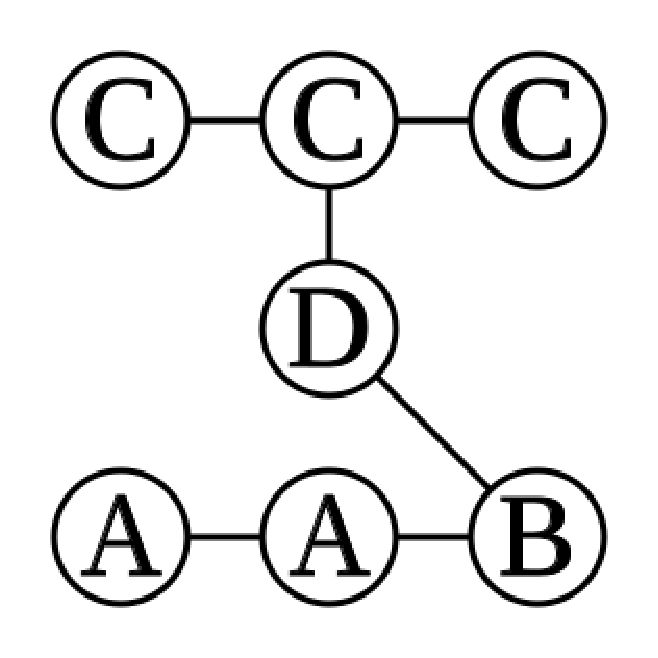
\includegraphics[width=0.4\textwidth]{img/artificial_graph/ccc2aab3.eps} \\
						$y = +1$
					\end{minipage} 
					\begin{minipage}{0.3\hsize}
						\centering
						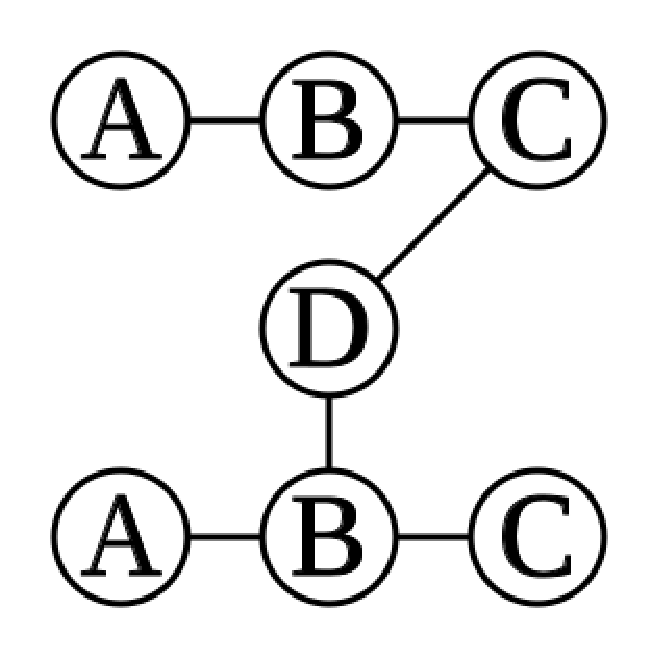
\includegraphics[width=0.4\textwidth]{img/artificial_graph/abc3abc2.eps} \\
						$y = -1$
					\end{minipage}
					\begin{minipage}{0.4\hsize}
						\centering
						\begin{tabular}{ll}
							\thickhline
							Group 1 & Group 2 \\
							\hline
							\gxxx{A}{A}{A} & \gxxx{B}{B}{B} \\
							\gxxx{C}{C}{C} & \gxxx{A}{A}{B} \\
							\gxxx{B}{C}{C} & \gxxx{A}{B}{C} \\
							\thickhline
						\end{tabular}
					\end{minipage} 
				\end{tabular}
			}
		\end{figure}

		\vspace{25pt}
		\begin{center}
			\express{非線形モデルが必要}
		\end{center}
		\begin{table}[t]
			\centering
			\scalebox{0.9}{
				\begin{tabular}{lll}
					\thickhline
					\multicolumn{1}{l}{\textit{非線形モデル}}~~~~~~~ &
					\multicolumn{2}{l}{\textit{線形モデル}} \\ \hline
					%Proposed & RF & Proposed ($d1$) & gBoost & LR \\
					提案手法 & 提案手法 ($d1$)~~~ & gBoost \\
					\hline
					%\fst{100.0} &  \scd{94.3}  & 64.3  & 70.0  & 53.9  \\
					~~\fst{100.0} & ~~~~64.3  & ~~70.0 \\
					\thickhline
				\end{tabular}
			}
		\end{table}
	\hspace{700pt} $d$: 木の深さ 

	\vspace{10pt}
	\structure{精度予測 (\%) QSAR} \\
	\vspace{-35pt}
	\begin{center}
		\express{実データに対しても高精度}
	\end{center}
	\begin{table}[t]
		\centering
		\scalebox{0.9}{
			\begin{tabular}{lcccc}
				\thickhline
				~                          &        CPDB                ~~~ &        Mutag             ~~~ &        NCI1               ~~~ &        NCI47                    \\ \hline
				\multicolumn{5}{l}{\textit{非線形モデル}} \\
				\ss{提案手法}{~}           &   \fss{79.3}   ~~~ &    \ss{87.8} ~~~ &   \fss{84.7}  ~~~ &   \fss{84.5}  ~~~   \\ \hline
				\multicolumn{5}{l}{\textit{線形モデル}} \\
				\ss{提案手法 (d1)}{~}      &    \fss{79.3}  ~~~ &    \ss{87.8} ~~~ &    \ss{83.1}  ~~~ &    \ss{82.8}  ~~~   \\
				\ss{gBoost}{~}             &    \ss{77.1}   ~~~ &   \fss{91.4} ~~~ &    \ss{82.7}  ~~~ &    \ss{81.3}  ~~~   \\
				\thickhline
			\end{tabular}
		}
	\end{table}

	\vspace{10pt}
	\structure{2-step 手法とのスケーラビリティの比較} \\
	\vspace{-35pt}
	\begin{center}
		\express{2-step手法よりもスケールする}
	\end{center}
	\begin{figure}[t]
		\centering
		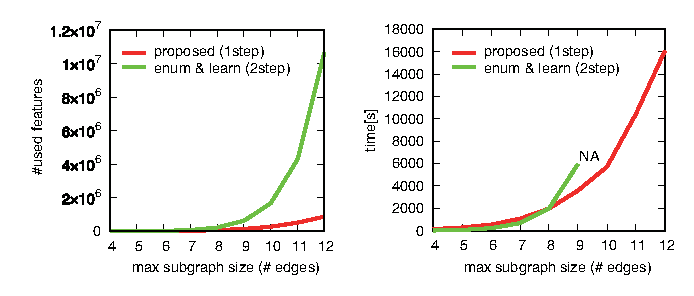
\includegraphics[width=1\textwidth]{img/fig7_panel.eps}
	\end{figure}
\end{tcolorbox}
